\begin{figure}[h]
\def\vertspace{1em}
\rotatebox{90}{\hspace{3em}Square map}%
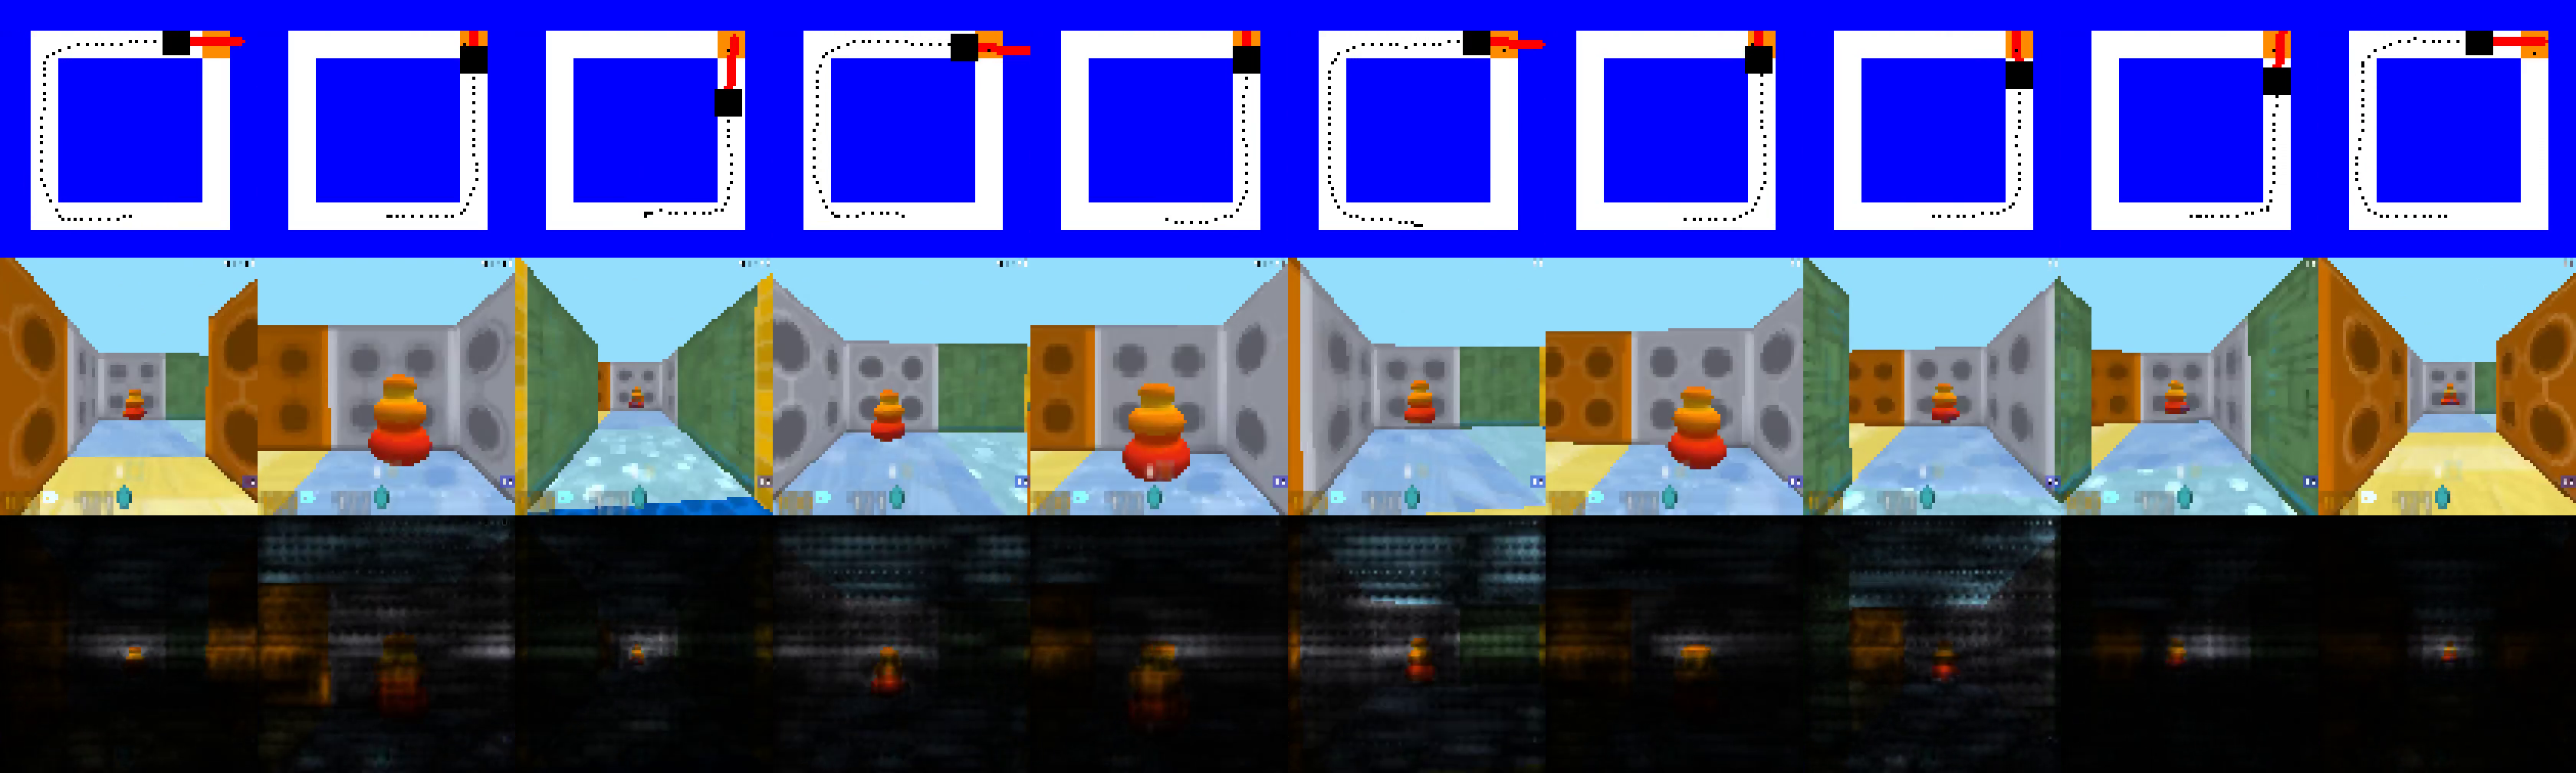
\includegraphics[width=0.98\textwidth]{./exp-results/training-1000_on_square_map.png}%
\vspace{\vertspace}
\rotatebox{90}{\hspace{4em}Wrench map}%
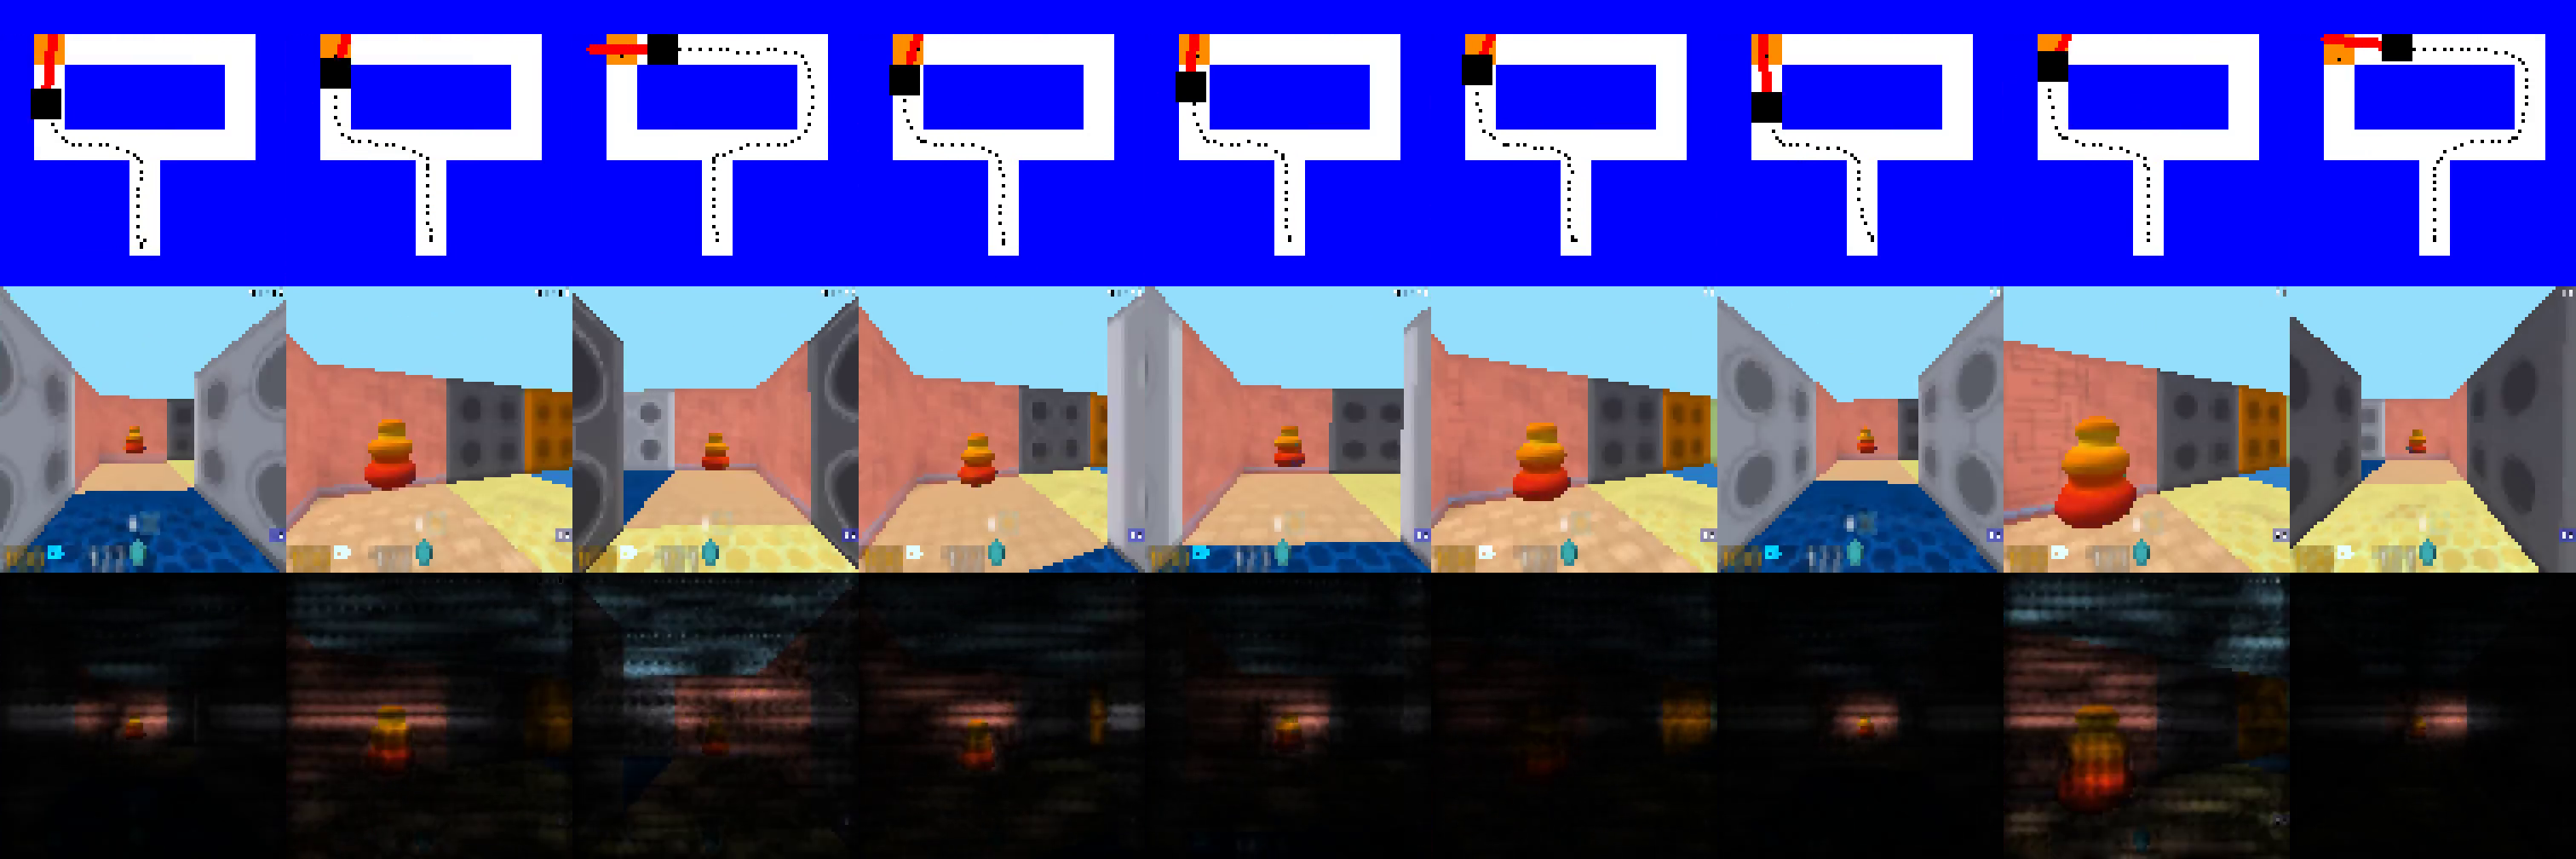
\includegraphics[width=0.98\textwidth]{./exp-results/training-1000_on_wrench_map.png}%
\vspace{\vertspace}
\rotatebox{90}{\hspace{5em}Goal map}%
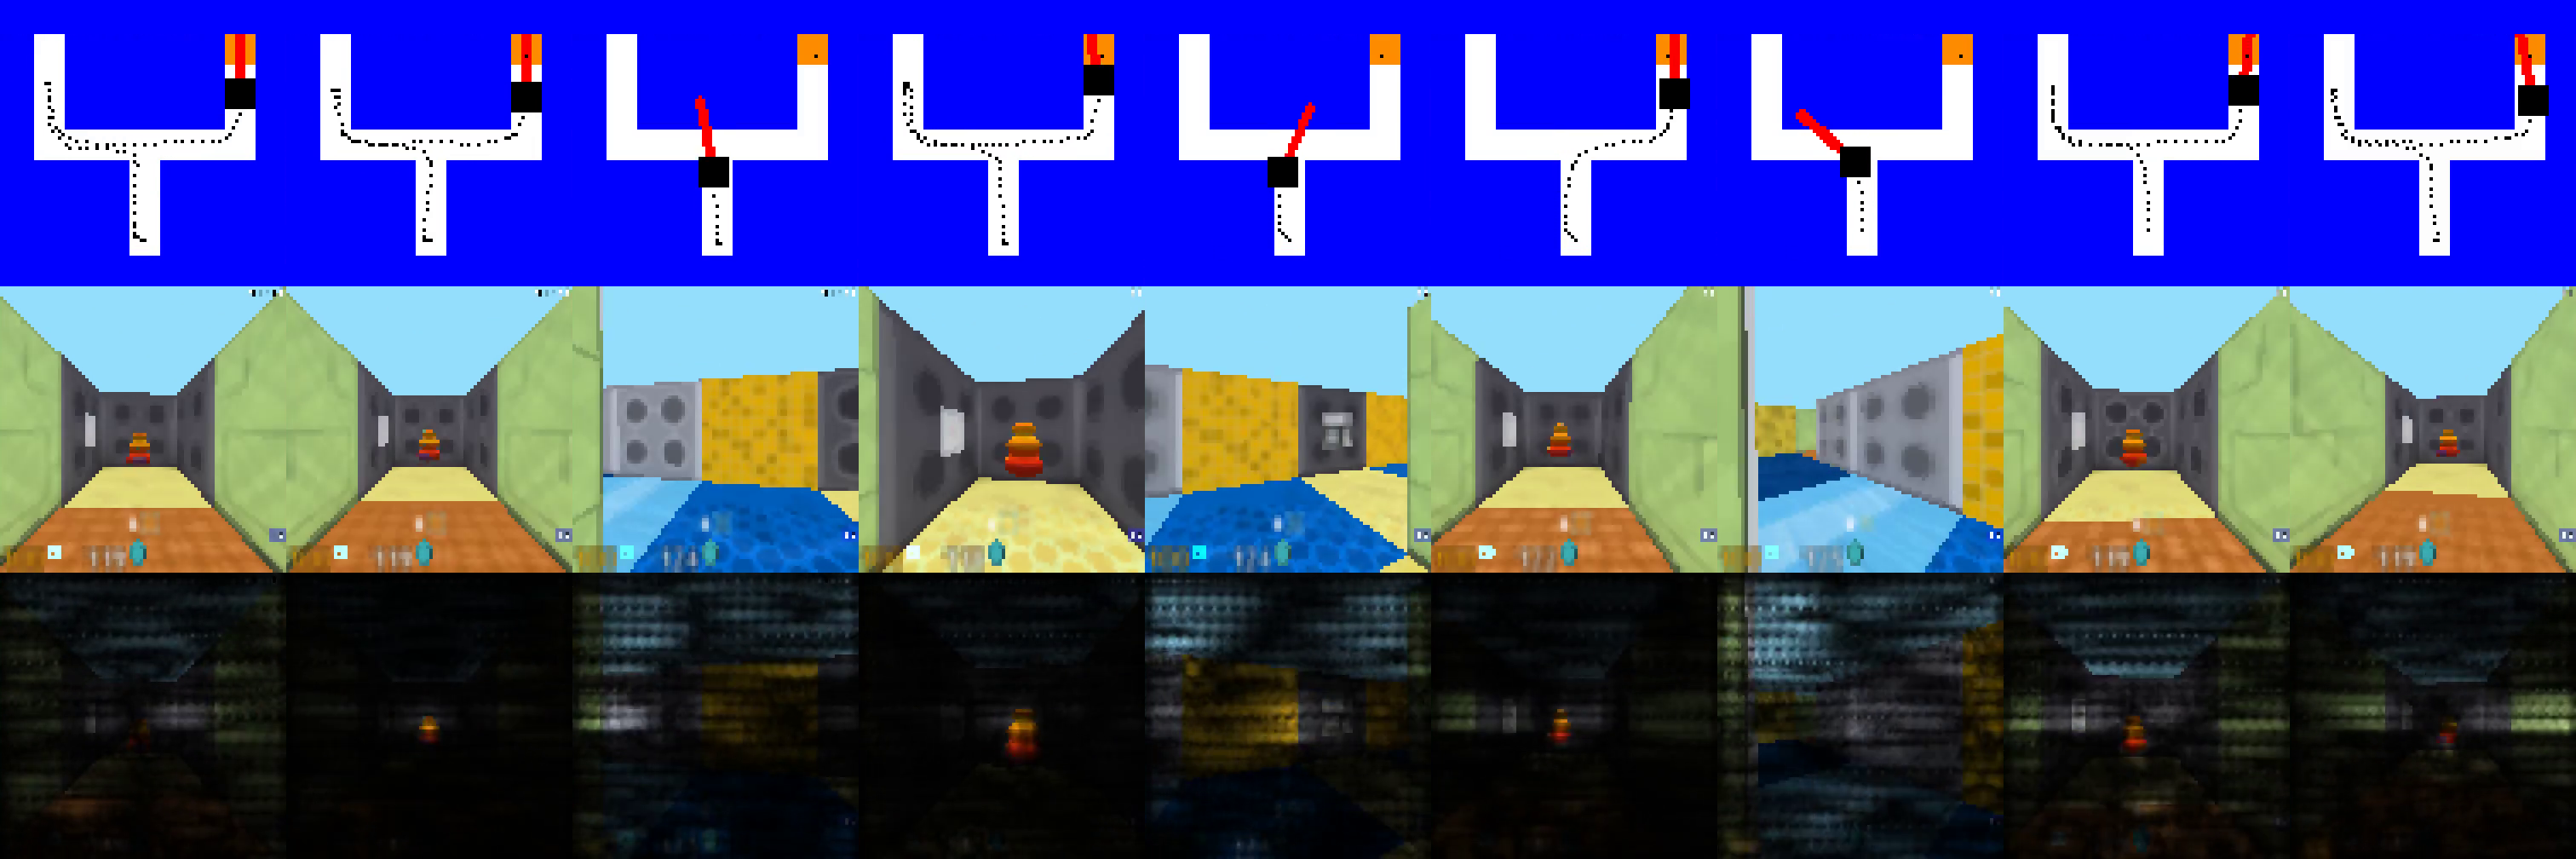
\includegraphics[width=0.98\textwidth]{./exp-results/training-1000_on_goal_map.png}%
\caption{Qualitative results when model trained on 1000 maps is
  evaluated on unseen simple maps.
  In this particular example, the agent takes the shortest path 6/10 times but when averaged over 100 episodes, the percentage of shortest path taken is reduced to $50.4$\% ($\pm 12.8$\%).
  Although for the example of wrench map the agent takes the shortest path 8/10 times but when averaged over 100 episodes, the percentage of shortest path taken is reduced to $32.9$\% ($\pm 25.1$\%).
 For the goal map, the example chosen here shows that the shortest path is only taken 1/6 times, on an average over 100 episodes, the shortest path is taken $42.6$\% ($\pm 35.1$\%) times.
}
\label{fig:planning-qualitative}
\end{figure}
